% THIS IS SIGPROC-SP.TEX - VERSION 3.1
% WORKS WITH V3.2SP OF ACM_PROC_ARTICLE-SP.CLS
% APRIL 2009
%
% It is an example file showing how to use the 'acm_proc_article-sp.cls' V3.2SP
% LaTeX2e document class file for Conference Proceedings submissions.
% ----------------------------------------------------------------------------------------------------------------
% This .tex file (and associated .cls V3.2SP) *DOES NOT* produce:
%       1) The Permission Statement
%       2) The Conference (location) Info information
%       3) The Copyright Line with ACM data
%       4) Page numbering
% ---------------------------------------------------------------------------------------------------------------
% It is an example which *does* use the .bib file (from which the .bbl file
% is produced).
% REMEMBER HOWEVER: After having produced the .bbl file,
% and prior to final submission,
% you need to 'insert'  your .bbl file into your source .tex file so as to provide
% ONE 'self-contained' source file
%
% Questions regarding SIGS should be sent to
% Adrienne Griscti ---> griscti@acm.org
%
% Questions/suggestions regarding the guidelines, .tex and .cls files, etc. to
% Gerald Murray ---> murray@hq.acm.org
%
% For tracking purposes - this is V3.1SP - APRIL 2009


\documentclass{acm_proc_article-sp}
%\documentclass{sig-alternate} 

\usepackage[utf8]{inputenc}
\usepackage{url}
\usepackage{float}
\usepackage{times}
\usepackage{color}
\usepackage[usenames,dvipsnames]{xcolor}
\usepackage{multirow}
\usepackage{listings}
\usepackage{times}
\usepackage{paralist}
\usepackage{wrapfig}
\usepackage{multirow}
\usepackage{ifpdf}
\usepackage{hyperref}
\usepackage[numbers, compress]{natbib}
\usepackage{array}

\begin{document}

\conferenceinfo{ECMLS'12,} {}
\CopyrightYear{2012}
\crdata{978-1-4503-0702-4/11/06}
\clubpenalty=10000
\widowpenalty = 10000

\newif\ifdraft
\drafttrue   
\ifdraft 
\newcommand{\jkimnote}[1]{{\textcolor{green} { ***Joohyun: #1 }}} 
\newcommand{\jhanote}[1]{ {\textcolor{red} { ***SJ: #1 }}}
\newcommand{\pnote}[1]{ {\textcolor{magenta} { ***Pradeep: #1 }}}
\newcommand{\rev}[1]{ {\textcolor{cyan} { ***reviewer1: #1 }}}
\newcommand{\secrev}[1]{ {\textcolor{Bittersweet} { ***reviewer2: #1 }}}
\newcommand{\alnote}[1]{ {\textcolor{blue} { ***andreL: #1 }}}
\newcommand{\todo}[1]{ {\textcolor{red} { ***TODO: #1 }}}
\newcommand{\fix}[1]{ {\textcolor{red} { ***FIX: #1 }}}
\newcommand{\ny}[1]{ {\textcolor{red} { ***NY: #1 }}}
\newcommand{\reviewer}[1]{} 
\else 
\newcommand{\reviewer}[1]{}
\newcommand{\jkimnote}[1]{} 
\newcommand{\pnote}[1]{}
\newcommand{\rev}[1]{}
\newcommand{\secrev}[1]{}
\newcommand{\alnote}[1]{}
\newcommand{\jhanote}[1]{}
\newcommand{\todo}[1]{}
\fi


\title{Understanding MapReduce-based Next-Generation Sequencing
  Alignment on Distributed Cyberinfrastructure}

%\title{Next-Generation Sequencing Reads Alignment Using Pilot-based SAGA-MapReduce}

\numberofauthors{3} %  in this sample file, there are a *total*
% of EIGHT authors. SIX appear on the 'first-page' (for formatting
% reasons) and the remaining two appear in the \additionalauthors section.
%
\author{
% You can go ahead and credit any number of authors here,
% e.g. one 'row of three' or two rows (consisting of one row of three
% and a second row of one, two or three).
%
% The command \alignauthor (no curly braces needed) should
% precede each author name, affiliation/snail-mail address and
% e-mail address. Additionally, tag each line of
% affiliation/address with \affaddr, and tag the
% e-mail address with \email.
%
\alignauthor Pradeep Kumar Mantha\\
       \affaddr{Center for Computation and Technology}\\
       \affaddr{Louisiana State University}\\
       \affaddr{216 Johnston}\\
       \affaddr{Baton Rouge, LA}
       \email{pmanth2@cct.lsu.edu}
\alignauthor Nayong Kim\\
       \affaddr{Center for Computation and Technology}\\
       \affaddr{Louisiana State University}\\
       \affaddr{216 Johnston}\\
       \affaddr{Baton Rouge, LA}
       \email{nykim@cct.lsu.edu}
\alignauthor Andre Luckow\\
       \affaddr{Center for Computation and Technology}\\
       \affaddr{Louisiana State University}\\
       \affaddr{216 Johnston}\\
       \affaddr{Baton Rouge, LA}
       \email{aluckow@cct.lsu.edu}
\and
\alignauthor Joohyun Kim\\
       \affaddr{Center for Computation and Technology}\\
       \affaddr{Louisiana State University}\\
       \affaddr{216 Johnston}\\
       \affaddr{Baton Rouge, LA} \\
       \email{jhkim@cct.lsu.edu}
\alignauthor Shantenu Jha\\
      \affaddr{Center for Autonomic Computing}\\
     \affaddr{Rutgers University}\\
      \affaddr{94 Brett Road}\\
      \affaddr{Piscataway, NJ}
     \email{shantenu.jha@rutgers.edu}
}
% There's nothing stopping you putting the seventh, eighth, etc.
% author on the opening page (as the 'third row') but we ask,
% for aesthetic reasons that you place these 'additional authors'
% in the \additional authors block, viz.
%\additionalauthors{Additional authors: John Smith (The Th{\o}rv{\"a}ld Group,
%email: {\texttt{jsmith@affiliation.org}}) and Julius P.~Kumquat
%(The Kumquat Consortium, email: {\texttt{jpkumquat@consortium.net}}).}
\date{25 Feb. 2012}
% Just remember to make sure that the TOTAL number of authors
% is the number that will appear on the first page PLUS the
% number that will appear in the \additionalauthors section.

\maketitle
\begin{abstract} 
  Although localization of Next-Generation Sequencing (NGS) data is
  suitable for many analysis and usage scenarios, it is not
  universally desirable, nor possible. However most solutions
  ``impose'' the localization of data as a pre-condition for NGS
  analytics.  We analyze several existing tools and techniques that
  use MapReduce programming model for NGS data analysis to determine
  their effectiveness and extensibility to support distributed data
  scenarios. We find limitations at multiple levels. To overcome these
  limitations, we developed a Pilot-based MapReduce (PMR) -- which is
  a novel implementation of MapReduce using a Pilot task and data
  management implementation.  PMR provides an effective means by which
  a variety of new or existing methods for NGS and downstream analysis
  can be carried out whilst providing efficiency and scalability
across multiple clusters.  
%Hierarchical MapReduce can be a viable
%  solution proposed for distributed data processing, but developing a
%  global reduce is not easy and straight forward in all cases and
%  might effect the statistical semantics of final output
%  data. 
Pilot-MapReduce (PMR) circumvents the use of global reduce and
  yet provides an effective, scalable and distributed solution for
  MapReduce programming model.  We compare and contrast the PMR
  approach to similar capabilities of Seqal and Crossbow, two other
  tools which are based on conventional Hadoop-based MapReduce for NGS
  reads alignment and duplicate read removal or SNP finding,
  respectively. We find that PMR is a viable tool to support
  distributed NGS analytics, particularly providing a framework that
  supports parallelism at multiple levels.
\end{abstract}

%   Next-generation DNA sequencing machines are generating enormous
%   amount of sequencing data, placing unprecedented demands on the
%   requirements of computational resources. MapReduce is proven as an
%   effective programming model to exploit the computational resources
%   efficiently for NGS data analysis.  A traditional single MapReduce
%   achieves parallelism at job(map and reduce) level, whilst most of
%   the workflows requires parallelism at MapReduce level i.e executing
%   multiple MapReduce instances concurrently, where a single cluster
%   does not provide enough resources to achieve significant performance
%   improvement. 


% -- fine grained
  % task-level concurrency for a wide range of NGS data analysis and
  % downstream processing.


% We analyze several existing tools and technqiues that use MapReduce
% programming model for Next-Generatiion Sequencing (NGS) data analysis.
% Our approach is based on the Pilot-based SAGA-MapReduce (PMR)
% framework which extends previously introduced SAGA-MapReduce with a
% Pilot task and data management implementation.  PMR provides an
% effective means to develop software tools with which a variety of
% existing or novel methods for NGS data and downstream analysis are
% carried out and more importantly achieve scalability across multiple
% clusters.  As demonstrating examples for the capabilities of our
% PMR-based approach, we implemented similar capabilities of Seqal and
% Crossbow, two other tools which are based on conventional Hadoop-based
% MapReduce for NGS reads alignment and duplicate read removal or SNP
% finding, respectively.  The comparison to these tools allows us to
% characterize our approach with PMR as a viable tool for the
% scale-across requirement as well as a versatile parallelism framework
% for a wide range of NGS data analysis and process tools.  The
% scalability with distributed sequencing data and the potentials for
% other analysis applications are discussed.


\category{D.1.3}{Software}{Concurrent Programming}{ Distributed
  programming/parallel programming} \category{J.3}{Computer
  Applications}{Bioinformatics, Mapping}


% A category with the (minimum) three required fields
%\category{H.4}{Information Systems Applications}{Miscellaneous} %Acategory including the fourth, optional field follows...
%\category{D.2.8}{Software Engineering}{Metrics}[complexity measures,performance measures]

\terms{Design, Experimentation, Performance}

 \keywords{Genome Sequence Alignment, BWA, Bowtie, Human Genome, RNA-Seq Data,
  MapReduce, Distributed Computing, Simple API for Grid
  Applications (SAGA), Pilot Job and Data}

%\keywords{ACM proceedings, \LaTeX, text tagging} % NOT required for Proceedings 
%\keywords{RNA conformation energy landscape, Runtime Environment, SAM-I riboswitch,
% S gene of Bovine Corona Viral Genome} % NOT required for Proceedings


% With astronomically explosive volumes of raw data and processed data,
% along with computational tasks that often need scalable
% infrastructure,
% computational implementations exploiting modern parallel processor or
% cluster architectures, and infrastructure developments
% altogether.

\section{INTRODUCTION} 

Recent advances in high-throughput DNA sequencing technologies such as
Next-Generation Sequencing (NGS) platforms have resulted in
unprecedented challenges in the areas of bioinformatics and
computational
biology~\cite{metzker2010,1000genome,wang2009-natrevgen,alex2009,mcpherson2009}.
These challenges are to some extent novel because of the need of the
cross-cutting and integrated solutions leveraging algorithmic
advances, tools and services, and scalable cyberinfrastructure and
middleware.

% As alluded to, MapReduce is a widely employed programming model for
% parallelization of a large data process; as reported by others with
% the tools listed in Table~\ref{table:mr-comparison},

% \jhanote{This does not fit here: The use of parallelism -- task-level,
%   thread-level and data-parallelism, continues to hold promise. In
%   fact, the programming model of MapReduce tries to exploit task-level
%   and data parallelism effectively.}

For dealing with unprecedented data and required data analytics and downstream analyses
of such high-throughput deep sequencing techniques, new strategies such as MapReduce-based
approaches have been added to an arsenal of computational biologists~\cite{schatz-nature-biotech-2010}.  Several tools using MapReduce have been already introduced for NGS data analysis such as read alignment onto a reference genome~\cite{cloudburst,
  gatk,langmead2009,seal2011,langmead2010, taylor2010}.

Since the paper about the MapReduce programming model from Google in
2004~\cite{mapreduce-2004-dean} and the emergence of Hadoop, the model
has drawn significant attention from various application domains as a
general strategy for parallelization of processing a large data.  Not
surprisingly, most of software tools using MapReduce for NGS data were
developed in the Hadoop environment and consequently with Cloud
computing environment such as Amazon EC2, consistent with the belief
that MapReduce implementations on Cloud environments provide an
efficient solution for big data
problems~\cite{mapreduce-2004-dean,schatz-nature-biotech-2010,
  taylor2010}.

Whereas the combination of MapReduce and Clouds works well for
scenarios where all ``the data can be poured into the Cloud'', often
this is not possible.  It is likely that the proportion/instances
where such stringent models of data localization are not possible will
increase.  Some contributing factors will be: increasing volumes of
data and thus greater challenge in transferring \& localizing it;
increasing number of data-repositories that will need to be accessed
-- each with their own data-transfer and access policies; greater
variety and distribution in the number of producers and consumers of
this data.

A consequence of the increasing importance of distributed data in NGS
analytics, is that current programming models -- or at least
programming models as currently implemented and executed, will prove
inadequate when faced with the challenge of distributed data; this
will be true of analytical approaches and tools that depend upon these
programming models. We thus posit that there is an emerging downstream
(analysis) problem in the field of NGS. 

While there have been algorithmic advances and a plethora of new
software tools providing user-friendly interface via web-based tools, client GUI, or integrative workbench environments \cite{galaxy}, the end-to-end
development of scalable infrastructure is lagging.  In other words,
it is still commonly observed that many biologists are puzzled by the proliferation of tools, and algorithms, whilst very few tools or solutions exist that are
extensible and flexible so as to yield integrated solutions.
 
The primary objective of our work is to demonstrate that existing
approaches can be extended to support distributed data scenarios with
simple but effective changes in their execution and runtime
environments.

Specifically, we demonstrate the use of a Pilot-based SAGA-MapReduce
with which NGS read alignments and subsequent analysis can be
conducted in a distributed, yet scalable fashion. Such Pilot-based
SAGA-MapReduce, herein referred to as PMR, can be thought of as the
capability resulting from writing MapReduce using SAGA to support task
and data distribution, whilst exploiting the capabilities of a
generalized and extensible Pilot-Job (and data) as a runtime
environment\cite{Sehgal2011590,pmr2012,pstar11}.

Before we discuss further contribution and outline of the paper, we
clarify our usage of the different types of scaling that this paper
will be concerned with: {\it scale-up} -- or the most common type of
scaling behavior, is a reference to the ability (performance) of using
many cores efficiently; {\it scale-out} is a measure of the number of
tasks that can be concurrently executed \& managed; {\it scale-across}
is a measure of the number of distinct compute resources that an
application can utilize.

Our experiments compare and contrast PMR with two known\\
MapReduce-based tools: Seqal in the Seal package and
Crossbow~\cite{seal2011,langmead2010}, for some features, including
but not limited to, i) scalability across multiple heterogeneous
infrastructures, ii) framework supporting extensions, iii)
effectiveness for data-intensive problem with distributed data.

% The two tools were used to carry out two different analyses; the
% alignment step was implemented as the first step with BWA and Bowtie,
% respectively but the second step was duplicate read removal for Seqal,
% whereas it was SNP finding for Crossbow.

%We observe that an efficient runtime environment for MapReduce such as
%that provided by PMR enables efficient methods for dealing with the
%required scalability of NGS data analysis which comprises short reads
%alignment and other following analysis such as duplicate read removal
%and SNP finding.  


The implementation of the MapReduce programming model using Pilot
capabilities in turn supports the development of applications which
have significant flexibility in scheduling as well as the ability to
exploit resources that are determined at runtime.  These features
(arising from the Pilot-abstraction) when coupled with
interoperability (arising from SAGA), enable such {\it dynamic
  applications}, to be executed across a range of distributed
resources -- such as clusters, or a mix of HPC grids and Clouds.

Indeed, based upon points (i) to (iii), PMR provides a viable compute
and data management environment for high-throughput DNA sequencing
data whilst using distributed cyberinfrastructure
effectively.  %PMR provides a viable approach for NGS data analytics.
We shall establish that in addition to providing solutions for challenges arising from the
required data volume scalability and efficiency, PMR can be a valuable approach 
for a broad range of NGS tools as well as the emergence of
revolutionary NGS techniques such as RNA-Seq.  It is instructive to
contrast the flexible and extensible support for such tools to other
approaches using Hadoop-based MapReduce
implementations~\cite{cloudburst,langmead2009,seal2011,langmead2010}.


% and computational requirements including the installation,
% maintenance, and update of the software tools.

% \jhanote{Say something about tooling, something about integrated the
%   concurrency also increased. and extensible environment}


% The comparison provides a promise for PMR tools combining the read
% alignment and successive tasks. 

Unfortunately, users cannot directly deploy a MapReduce framework such
as Hadoop on top of these clusters to form a single larger MapReduce
cluster. Typically the internal nodes of a cluster are not directly
reachable from outside. However, MapReduce requires the master node to
directly communicate with any slave node, which is also one of the
reasons why MapReduce frameworks are usually deployed within a single
cluster. Therefore, one challenge is to make multiple clusters act
collaboratively as one so it can more efficiently run MapReduce \cite{ecmls11-mr-autodock}.
 
Hierarchical MapReduce as proposed in~\cite{ecmls11-mr-autodock} is
often a viable solution to the distributed data problem, but
developing a global reduce is not easy and straightforward in all
cases. Indeed, many analyses for NGS data are not appropriate for Hierarchical MapReduce. 
On the contrary, PMR~\cite{pmr2012} is a distributed solution and
circumvents the use of a global reduce, providing an efficient and scalable solution for MapReduce applications. 

The paper is organized as follows. In
Section~\ref{sec:materials_and_methods}, the data sets we used for
this work and experimental methods are described.
%In Section~\ref{sec:experiments}, we describe the rational and experimental details for this paper. 
After that, in Section~\ref{sec:results}, our results for parallel performance
measurements and comparison of PMR with Seqal and Crossbow
which represent applications that use the open source Hadoop-based
MapReduce\cite{hadoop-url, taylor2010,seal_2011_mapred,seal2011} are
presented.  Finally, in Section~\ref{sec:discussions}, we 
discuss and conclude this paper with remarks focusing on
implications of our work for the development of biological
information infrastructure around NGS data.  
% for a short term goal of
%RNA-Seq data analysis and for a long term goal for an integrative
%research infrastructure that provides various holistic services of
%downstream analyses streamlined with effective computation of NGS data
%and analytics.

\begin{center}
\hfill{}
\begin{figure*}
 \centering
%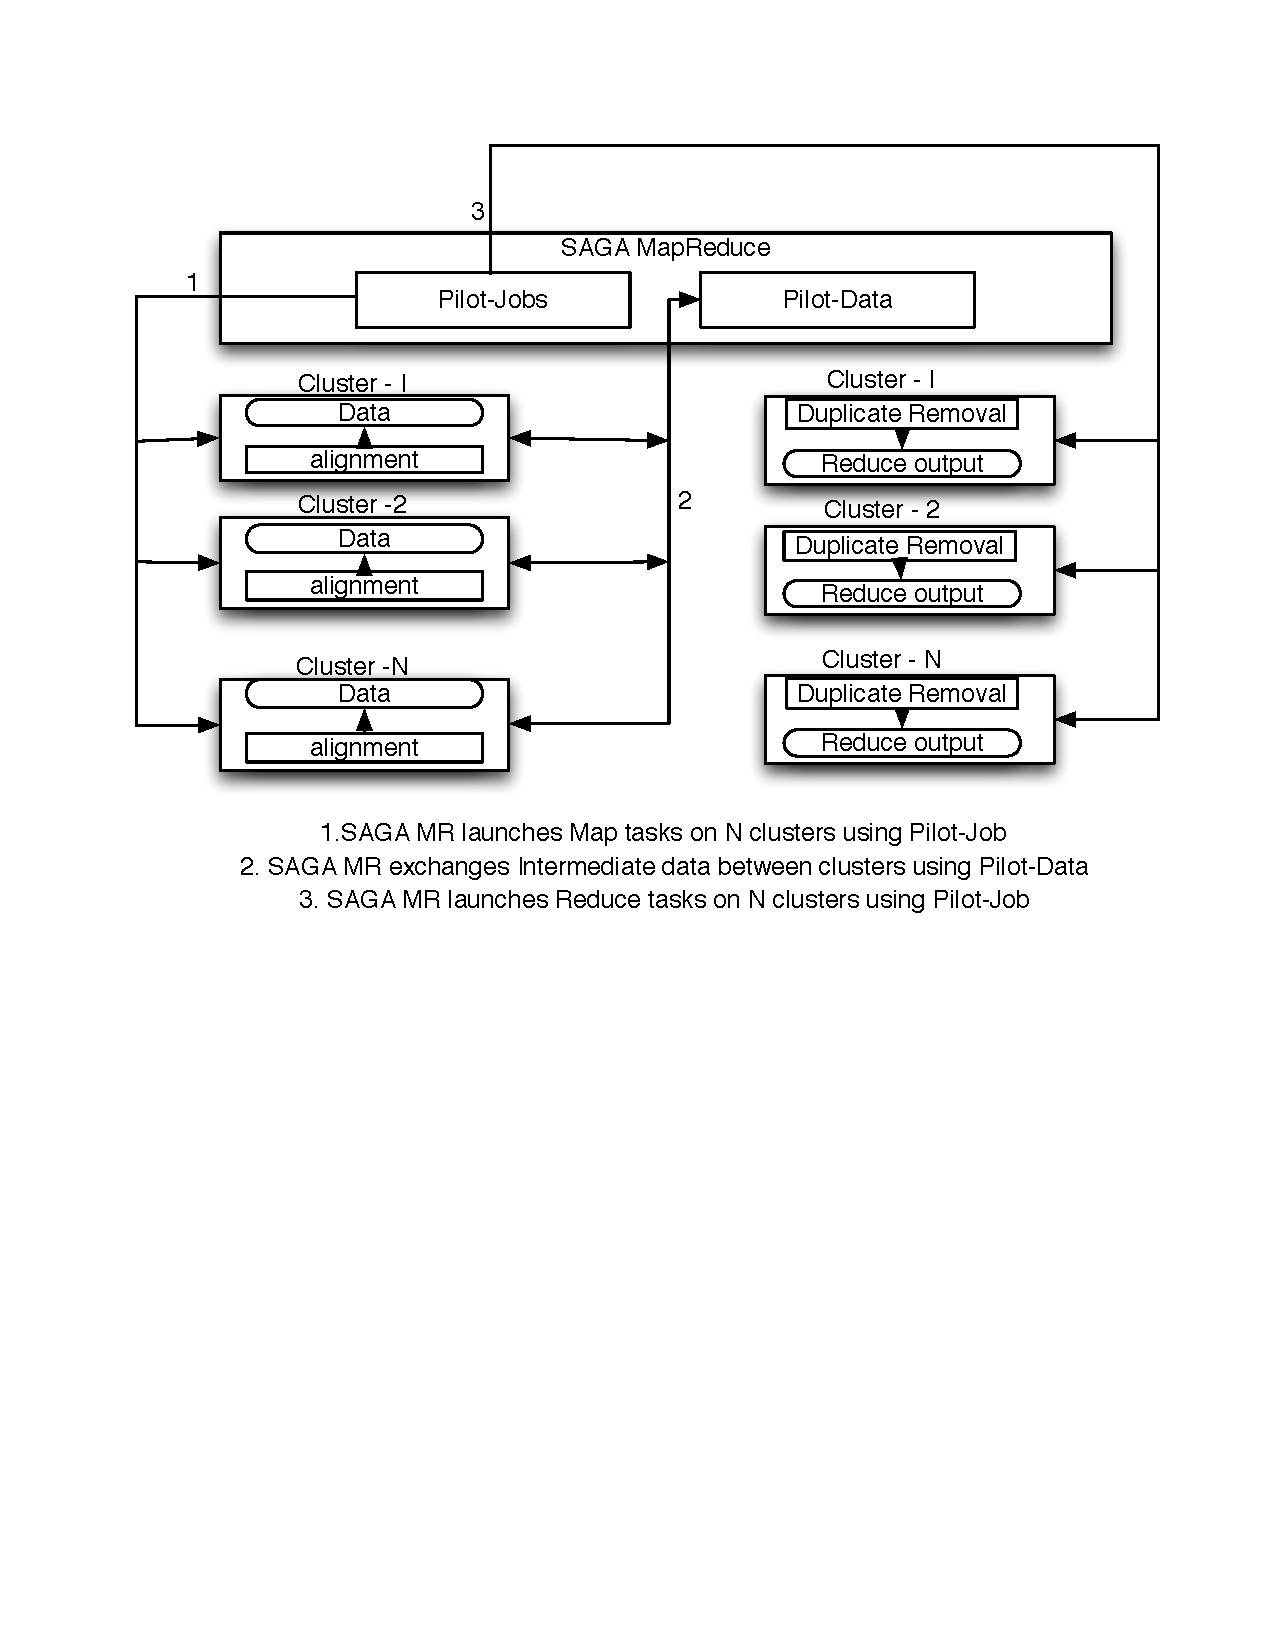
\includegraphics[scale=0.45]{figures/align-dup.pdf} 
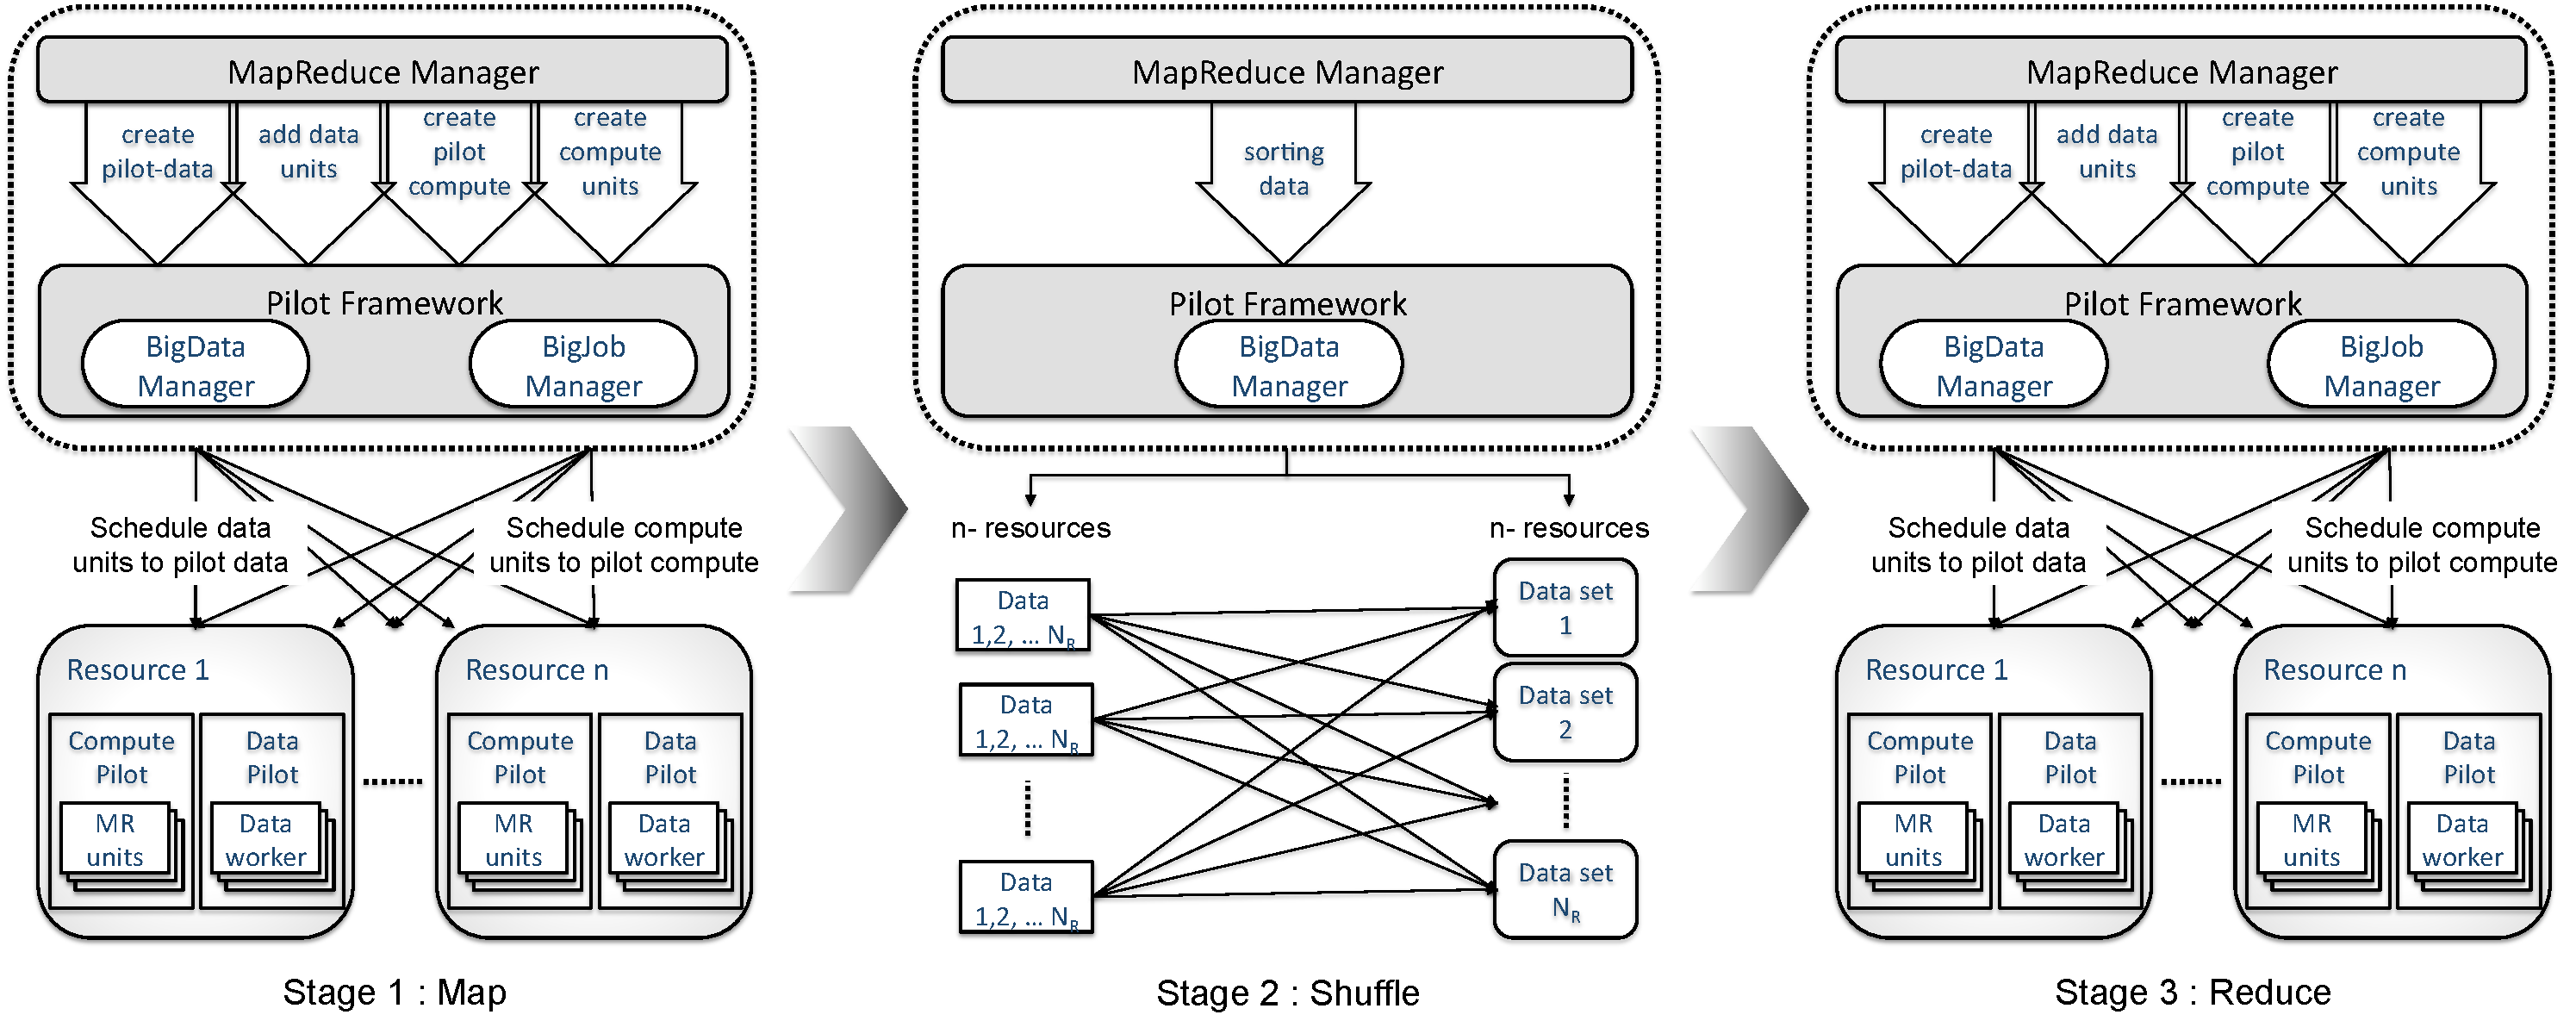
\includegraphics[scale=0.35]{figures/F1_1.pdf} 
\hfill{}
\caption{\small PMR architecture and the workflow for a MapReduce task: The compute and data units are basic blocks of scheduling in Pilot abstractions ~\cite{pstar11}. In our NGS analysis, the compute units in map phase are the alignment tasks, data units in the shuffle phase refer intermediate data units generated and compute units in reduce phase could be either duplicate read removal or SNP finding tasks.}
  \label{fig:arch-pj-saga-mr} 
\end{figure*}
\end{center}


\section{Materials and Methods}\label{sec:materials_and_methods} 
\secrev{It would also be useful for the paper to describe a few more details of Pilot and SAGA -- most significantly, are they open source and freely available so that they can be deployed as easily as Hadoop can be? What other requirements do they have?}

In this section we explain the materials and methods used for our NGS data analysis used by PMR and other Hadoop based applications.

\subsection{NGS Data Sets}
We used paired-end RNA-Seq data from the Flemington lab, from a Human
Burkitt's lymphoma cell line~\cite{erik_2010}. The read length is 100
for both directions of paired-end data, and the total size of each
data set is about 20.1 GB containing 70,927,422 reads.  For varying
size of sequencing data experiments, we chunked the required amount of
reads by partitioning the entire data.  For example, 2 GB paired end
data implies 1 GB for one end and 1 GB for the other end.  The file
format of sequencing data is fasta and all manipulation of sequencing
data was conducted by in-house python scripts and
samtools~\cite{samtools}. The reference genome is indexed based on the alignment tool
used and pre-staged to the machines before read mapping is performed.

\subsection{HPC Resources}

For this work, we used two Futuregrid systems -- Sierra and Hotel.
More details on the specification of these machines can be found from
the web page of Futuregrid~\cite{futuregrid_url}.  In brief, two
systems are multi-node clusters and equipped with the PBS job
scheduler and Hadoop, implying that the systems are appropriate to
test our PMR and to compare our results with Hadoop-based
tools. Hadoop version 0.20.2 was used with the two FutureGrid
machines. A replication factor of 2 and default chunk size of 128 MB
is used.

\subsection{File Systems}

In our experiments, both PMR and Hadoop are executed on a shared file system.
A shared file system is a common file system accessible for all the compute nodes on a single cluster.
Hadoop performs well when compute node local disks are used to build HDFS, but due to limited local disk space of compute nodes we utilized shared file system to build HDFS. 
PMR utilize the shared file system to read/write the data, whereas Hadoop uses HDFS to read/write the data, which is built on the same shared file system.

\subsection{Pilot-MapReduce (PMR)}

Pilot-MapReduce is a pilot-based implementation of the MapReduce
programming model, which decouples the logic/pattern of MapReduce from
the actual management of the compute, data and network resources. By
decoupling job scheduling and monitoring from the resource management,
PMR can efficiently reuse the resource management and late-binding
capabilities of BigJob and BigData.

PMR exposes an easy-to-use interface which provides the complete
functionality needed by any MapReduce-based application, while hiding
the more complex functionality, such as chunking of the input, sorting
the intermediate results, managing and coordinating the map and reduce
tasks, etc., these are generically implemented by the
framework~\cite{pmr2012}.  

PMR supports different MapReduce topologies (i) \emph{local} (ii)
\emph{distributed} (iii) \emph{hierarchical}. Local PMR performs all
map and reduce computations on a single cluster.  Distributed and
hierarchical PMR are mainly intended to support distributed data
processing without a need of global file system between multiple clusters.

Distributed PMR performs map tasks on the multiple resources close to
the initial input data and moves the intermediate data files to
another resource for executing reduce tasks. In hierarchical PMR the
output of first phase of MapReduce are combined using final MapReduce
step. We showed the relative advantages between hierarchical PMR and
distributed PMR in Ref.~\cite{pmr2012} based on the type of workload
or data aggregation involved. In this work, we mainly focus on local
and distributed PMR.  Fig.~\ref{fig:arch-pj-saga-mr} illustrates the
MapReduce flow using PMR.

\begin{itemize}
\item{~PMR launches map tasks on N clusters using the Pilot-Job of Pilot framework.}
\item{~After the map stage, PMR shuffles intermediate data between clusters using Pilot-Data of Pilot framework} 
\item{Finally,PMR launches reduce tasks on a cluster using the Pilot-Job of Pilot framework.}
\end{itemize}

\subsection{Target NGS Analysis}

In this section we present the important steps of DNA sequencing that
we consider for our work.

\subsubsection{Short Read Alignment}

Short reads alignment and the de-novo assembly are the required first
steps in every pipeline software tool that aims to support sequencing
data from NGS platforms.  De-novo assembly still remains a challenge,
because of complications arising from the short length of sequencing
reads from NGS machines. In practical sense, read alignment or mapping
is considered as the first task of most of the NGS
workflows. 

Generally for RNA-Seq data analysis, in particular with eukaryote
genomes, the spliced aligner such as TopHat~\cite{pepke2009} is
used. In our work, we consider an alternative strategy, to use a
non-spliced aligner and later splicing events are detected separately,
justifying the use of non-spliced aligners such as BWA and Bowtie for
the RNA-Seq data. We consider non-spliced aligner tools, Bowtie and
BWA tools to align short reads onto human reference genome hg19.

\subsubsection{Post-Alignment}
Duplicate read removal step might be required after short read
alignment, because sample preparation processes before sequencing
might contain artifacts stemming from high-throughtput read
amplification; many duplicates introduced are not relevant to true
biological conditions. 

Seqal is a Hadoop MapReduce application which implements the alignment
in map phase using BWA aligner and the same criteria as the Picard
MarkDuplicates~\cite{seal2011,seal_2011_mapred} for duplicate read
removal in reduce phase.  On the other hand, information about aligned
reads is essential for many downstream analyses such as SNP finding, 
genome variation study, transcriptome analysis, complex functional
genomics and pathway analysis. 
% Crossbow is a Hadoop streaming-based
%MapReduce application which performs alignment in the map phase using
% Bowtie aligner and performs SNP finding in the reduce phase
Crossbow ~\cite{langmead2009} is a scalable software automatic pipeline, combines Alignment and SNP finding tools for genome resequencing analysis.
Crossbow contains 4 steps - preprocessing, Alignment, SNP finding and postprocessing.  Each step is a Hadoop streaming based MapReduce application and the output of each step is stored in HDFS and read from HDFS by next step. In our experiments we focused on Crossbow alignment which uses Bowtie aligner in map phase and has zero reduces.  

%Interestingly, Crossbow uses Bowtie aligner and thus our PMR-based tool is extended to utilize Bowtie, in addition to BWA for the comparison with Crossbow.  Note that Bowtie is well-known for its %efficiency in memory requirement and computation, but the current version do not support gapped alignment whereas BWA does.}

\subsection{Experiments: Motivation and Configuration}

% The primary goal of our work is to provide a scalable and extensible
% MapReduce runtime framework capable of supporting various steps of
% sequencing procedure.

\rev{Discussion.  The paper does not discuss how the reference genome is distributed and how/when it is indexed.  This is a concern for smaller data sets and large genomes (although the granularity here of ~1 hour jobs should make this negligible).}

Our experiments compare PMR-based approach with Hadoop API based Seqal
%(tool for alignment and duplicate removal) 
and Hadoop streaming based Crossbow 
%(tool for alignment and SNP finding) 
(see Table 1) to:

\begin{itemize}

\item{Compare scale-out, scale-up and scale-across (as applicable) on
    distributed cyberinfrastructure using various NGS analytic tools}

\rev{The authors should not discuss "scale across" as they only used one platform (FutureGrid) and many of their comparisons relied on a shared file system given limitations of the disks.  This would be fixed by using more cores (32 max is relatively low, especially as "common" servers are approaching 16+ cores).  Also, how data is transferred can be important especially when the clusters are present at different institutions (say with Condor).}

\item{Investigate extensibility to support multiple NGS analytic
    tools}
\item{Compare PMR support for fine and coarse grained parallelism}.
\end{itemize}

Seqal and Crossbow are different from other tools such as Cloudburst
and GATK (as summarized in Table~\ref{table:mr-comparison}), in terms
of usage and the type of parallelism they employ for NGS data
processing and management.

%Seqal performs short read alignment using BWA aligner in map phase and
%duplicate read removal in reduce phase.  Crossbow performs short read
%alignment using Bowtie aligner in map phase and SNP finding in reduce
%phase using SOAPsnp. \pnote{repeated}

For our experiments, Seqal part of Seal package
of version 0.2.3 version and Crossbow package of version 1.1.2 is
used. Crossbow 1.1.2 uses Bowtie 0.12.7v and SOAPsnp 1.02v
tools. Default configuration or execution options are used for both
the packages.

Preprocessing is a common step for both Seqal and Crossbow. The input
file format for Seqal is prq format.  We use PairReadsQSeq tool of
Seal package to convert qseq/fasta format files to prq
format. Crossbow also performs preprocessing on input fast files and
then performs alignment, snp finding. 

We developed a PMR based NGS applications which are similar to Seqal
and Crossbow. PMR based approach for Seqal involves developing a
custom map script which performs short read alignment using BWA
aligner and reduce script to perform duplicate read removal based on
the same criteria provided in~\cite{seal_2011_mapred}. But the reduce
phase implementation significantly vary from the seqal
implementation's. PMR based approach for Crossbow  alignment step 
involves development of a custom map script which performs short read alignment using
Bowtie aligner. 

\pnote{commented -Currently, we focused only on comparision of PMR based approach with alignment step of Crossbow, 
we will investigate and compare the SNP finding step performance in our future work.}

When executing Hadoop based MapReduce NGS tools on production
cyberinfrastructure, we request a set of nodes to start the Hadoop
cluster. Once required resources are obtained, we set the number of
map and reduce tasks per node and number of nodes
($N_{W}/node$)~\jhanote{need better notation..} via Hadoop
configuration or NGS analytic tool configuration.  Once the Hadoop
cluster is ready, NGS tools can be executed. Hadoop MapReduce
environment setup involves significant amount of efforts and it is not
trivial for a new user.

PMR provides a simple framework which can be easily deployed on
multiple clusters. PMR inherits the advantage of Pilot abstractions
which liberates the application/user from the resource
management. Some of the parameters involved in PMR setup are
specifying the map and reduce scripts and their arguments, number of
cores for each map and reduce task, total number of compute nodes for
entire MapReduce application and the maximum estimated time (wall
time) required to run the MapReduce, nature of the map or reduce task
(single or mpi).

There is no limitation on the number of cores that can be assigned to
a map/reduce task, where as Hadoop places a hard-limit on the number
of cores on a map task as the number of cores per node. This affects
the performance of the MPI based NGS tools which scale-up well. For
example NovoalignMPI~\cite{novo-align} is a message passing version of
Novoalign, with claims of being one of the most accurate aligners,
allows a single alignment process to spread across mutliple compute
nodes.

The default input split/chunk size used by Hadoop based applications
is 128MB. In the PMR based applications, we make sure the right amount
of chunk size is specified so that the number of map tasks are equal
in both Hadoop and PMR approaches. The chunk size for PMR is
considered as number of reads. The number of mappers($N_M$) depend on
the size of input($S_I$) and chunk size. The number of reduces($N_R$)
is set to 8 in our experiments. For the relation between parameters
used for the experimental set-up, see examples in
Table\ref{table:exp-description}.

PMR based applications directly use the fasta format files and no
preprocessing required.  The intermediate data management affects the
performance of NGS tools in distributed data processing. PMR uses
Pilot-Data which transfer the intermediate data in parallel and across
multiple clusters. Hadoop depends on HDFS and TCP/IP based
communication between data nodes.

\begin{center}
\begin{table*}[ht]
{\small
\hfill{}
\begin{tabular}{|l|l|c|c|c|c|c|c|}
\hline
  &\centering \textbf{PMR}\cite{pmr2012} & \textbf{Seqal}\cite{seal2011} & \textbf{Crossbow}\cite{langmead2009} & \textbf{CloudBurst}\cite{cloudburst} & \textbf{GATK}\cite{gatk} \\ \hline
%\cline{3-9}
 \hline 
 Key Parallelism   & Pilot-based   &  Hadoop-based/  &  Hadoop   & Hadoop-based & MR-based Structured \\ 
Strategy  & Distributed MR & MR  & Streaming  & MR & Programming  \\
& & (Pydoop) &  & & Framework \\ \hline
  
Hadoop & No & Yes & Yes\footnote[1] & Yes & No \\ 
Requirement  & & & &  &\\ \hline  
    
Multiple  Cluster & Yes  & Limited   & Limited  & Limited  & Limited \\
Support &  & by Hadoop &  by Hadoop & by Hadoop  & by JVM   \\ \hline

Multiple Node & Support & Not allowed  & Not allowed  & Not allowed & Not  \\
Task Supprt &  & by Hadoop & by Hadoop & by Hadoop & Easy  \\ \hline
Distributed Job and  & Advert Service  & Hadoop/HDFS & Hadoop/HDFS & Hadoop/HDFS & Java \\ 
Data Coordination &(SAGA) &  & & & Framework\\ \hline


Primary Aligner &  BWA, Bowtie,  &  BWA & Bowtie & RMAP &  BWA \\
& and Others (coming) &  &  &  &  \\ \hline
Multiple Aligner  & Straightforward & Not Straight- & Possible & Not Straight-  & Straight-  \\ 
Support &  & forward &   & forward  & forward \\\hline
Primary Tasks & Alignment/Duplicate  & Alignment/ & Alignment/ & Alignment &Various\\
  &  Removal & Duplicate & SNP Discovery & & NGS Data  \\  
           & (and Extensible &  Removal & &  & \& Downstream  \\
           & for RNA-Seq) & & &  & Analysis \\ \hline  
Extensibility for   &  High  & Medium &  Low & Low & High      \\
Multiple Tools  &      &  &  &  &   \\ \hline

\hline
\end{tabular}}
\hfill{}
\caption{Feature comparison of PMR with other tools for NGS data analysis that primarily provide a parallelism support using the MapReduce framework.  $^{1}${The feature of Crossbow that can run with a desktop environment without Hadoop is not considered in the scope of this work due to the lack of scalability support.} }
 \label{table:mr-comparison}
\secrev{Finally, Table 1 should be updated - Crossbow is very extensible, and the Crossbow code forms the basis for the RNAseq analysis pipeline Myrna published in 2010: http://genomebiology.com/2010/11/8/R83}
\end{table*}
\end{center}

%\subsubsection{Comparing  Seqal and Crossbow}

\begin{center}
\begin{table*}[ht]
\small
\hfill{}
 \begin{tabular}{|c|c|c|c|c|} 
 \hline 

 \textbf{Case} &  \textbf{ \# of  Nodes ($N_{node})$ :}  &  \textbf{\# of Workers} &   \textbf{\# of Mappers} & \  \textbf{Related Experiments} \\
 \textbf{E($N_{node}$, $N_W$,  $N_M$)} &  \textbf{Total \# of cores} &   ($N_W$)  & ($N_M)$  &  \textbf{ in Figure (case)}  \\
 \hline
  \hline
E(2,4,13) &2 : 16 & 4 & 13 & Fig 6(2 nodes) \\
E(4,8,32) & 4 : 32 & 8 & 32 & Fig 3(4 nodes) \\
E(4,8,13) & 4 : 32 & 8 & 13 & Fig 5(2GB read size), Fig 4(upper-2GB read size) \\
E(4,8,25) & 4 : 32 & 8 & 25 & Fig 5(4GB read size), Fig 6(4 nodes), Fig 4(upper-4GB read size) \\ 
E(4,8,50) & 4 : 32 & 8 & 50 & Fig 5(8GB read size), Fig 4(upper-8GB read size), Fig 4(lower)\\ 
E(8,16,32) & 8 : 64 & 16 & 32 & Fig 3(8 nodes)\\ 
E(8,16,50) & 8 : 64& 16 & 50 & Fig 6(8 nodes)\\ 
E(16,32,32) & 16 : 128 & 32 & 32 & Fig 2(10GB read size), Fig 3(16 nodes)\\ 
E(16,32,64) & 16 : 128 & 32 & 64 & Fig 2(20GB read size)\\ 
E(16,32,128) & 16 : 128 & 32 & 128 & Fig 2(40GB read size)\\ 

%Case & \# of  & \# of &  \# of & \# of & \# of  \\
%E($N_{node}$,$N_W$,  & Nodes & Worker   & Mapp- & Reduc- & available  \\
%$N_M$, $N_R$,  & &  & ers & ers & cores per\\
%$S_I$ (GB)) & ($N_{node})$& ($N_W$) & ($N_M) $ & ($N_R$) & Worker \\
%\hline
%E(4, 4, 32, 8, 8) &4 &  4 & 32  & 8 & 8 \\
%E(4, 8, 32, 8, 8) & 4 & 8 & 32 & 8 & 4 \\
%E (8, 8, 32, 8, 8) & 8 & 8 & 32 & 8 & 8 \\ 

 \hline
 \end{tabular}
 \hfill{}

\rev{Also, the last column in Table 2 does not match the legend as all nodes have 8 cores (and therefore 8 cores are only available with one worker per node?).  Figures 2 and 3 do not have entries in Table 2 (specifically the 16 node job).}

 \caption{Description of experimental cases examined in this paper for understanding scalability, impact of parallelism strategy, and performance comparison.  A experiment will be described with the three parameters in E($N_{node}$,$N_W$,$N_M$).  The related experiments in figures are illustrated in this table.  Note that all nodes for this study have 8 cores, 8 reducers and the number of cores per Worker is determined by the total number of cores divided by the number of Workers in a node.}
    \label{table:exp-description} 
\end{table*}
\end{center}

\section{Experiments and Evaluation}\label{sec:results}

We evaluate the performance of the PMR-based applications in the
context of scalability at different levels and extensibility to
multiple tools.  Each experiment is repeated at least three times.

\subsection{Scalability}

PMR runtime involves time taken to chunk the input data, map, shuffle
and reduce phase times.  The scalability characteristics of PMR, for
different levels of parallelism and granularity were evaluated using
applications specified in Section~\ref{sec:materials_and_methods}.  

In the first experiment shown in the Fig~\ref{fig:read-size}, not
surprisingly the total runtime increased linearly as the input read
size increased. PMR \textit{scales-out} well as the number of compute tasks increase on 16 nodes(128 cores).

Fig ~\ref{fig:scale-p-saga-mr} shows how PMR \textit{scales-up}. PMR
scales-up well as the runtime decreases with increase in number of
nodes.

In both, the map phase (read alignment) is a single dominant step for
the overall time-to-solution, and the reduce task (duplicate read
removal) is relatively less compute intensive task. The intermediate
data is managed by Pilot-Data which parallelizes the intermediate data
transfers between map and reduce phases in a cluster or between
clusters, which improves performance of PMR.

Fig ~\ref{fig:comp_with_seqal_1} shows the comparison of different
configurations of PMR with Seqal application.  The setup phase for Seqal involves
copying of the reference archieve to all the data nodes and extracts it so it is available locally,
whereas the setup phase for PMR involves chunking of data. Notably, Seqal takes more time than other configurations of PMR because of the reason that
HDFS is build on shared file system. The local disks of compute nodes available on FutureGrid are
too small for the used input data; thus, HDFS had to be configured to
utilize a shared file system, which leads to a
non-optimal performance during the I/O intensive map phase.


Hadoop is a prominent framework for doing MapReduce computations but it is
designed for cluster/local environment, but not for a high degree of
distribution. Unfortunately, Hadoop cannot be executed on more than
one cluster on Futuregrid, because of firewall issues.Hierarchical MapReduce~\cite{ecmls11-mr-autodock} provides a viable
solution to use multiple clusters for MapReduce programming model and
then combine the final output with a global reduce function. Designing
global reduce is not easy and straightforward in all cases. For
example in Crossbow application, combining reduce outputs of multiple
SoapSNP's using a global reduce might effect the semantics of the
final data. The distributed PMR could be a viable solution for running
MapReduce programming model on multiple clusters without a global filesystem between the clusters. Distributed PMR
is executed on Sierra and Hotel, where the number of workers and the
input data is distributed equally between the machines.

Distributed PMR performs significantly better than Hadoop Seqal, but
it is slower than local PMR; this is attributable to the overhead of
distributing tasks between the machines.  But this overhead is
significantly less important than the advantages of
\textit{scaling-across} is considered which allows concurrent usage of
multiple cluster resources. The other reason is that the time taken to transfer intermediate data from Hotel to Sierra by Pilot-Data, which is produced by the map phase on Hotel.
 Once the entire intermediate data is available the reduce phase is executed on Sierra. 

Note that the direct comparison of the reduce phase is not straightforward due to the potentially different
implementation between Seqal and our custom duplicate read removal reduce function \jhanote{what is ours. please
 replace with whatever ours is!!}\pnote{addressed}, in spite of the fact that the same
criteria of duplicate read removal of Seqal\cite{seal_2011_mapred} was
used. The map phase of Seqal and PMR tool are almost comparable since
the same aligner, BWA is used and all parameters (see
Table~\ref{table:exp-description}) for configuring a MapReduce task
are same in the comparison.

%The computation of read alignment and duplicate read removal represents an
%interesting and simple category of computational tasks among NGS data
%analysis that could be benefitted by employing the MapReduce
%programming model.  We implement such a MapReduce task with PMR.  The
%main findings with this analysis are as follows.  First, as shown in
%Fig.~\ref{fig:read-size}, the scalability is critically required as
%the input data size increases.  Not surprisingly, the results shown in
%Fig~\ref{fig:scale-p-saga-mr} suggests that the parallel strategy with
%MapReduce could be a viable solution for increasingly demanding large
%data sets.

 \begin{figure}
 \centering
%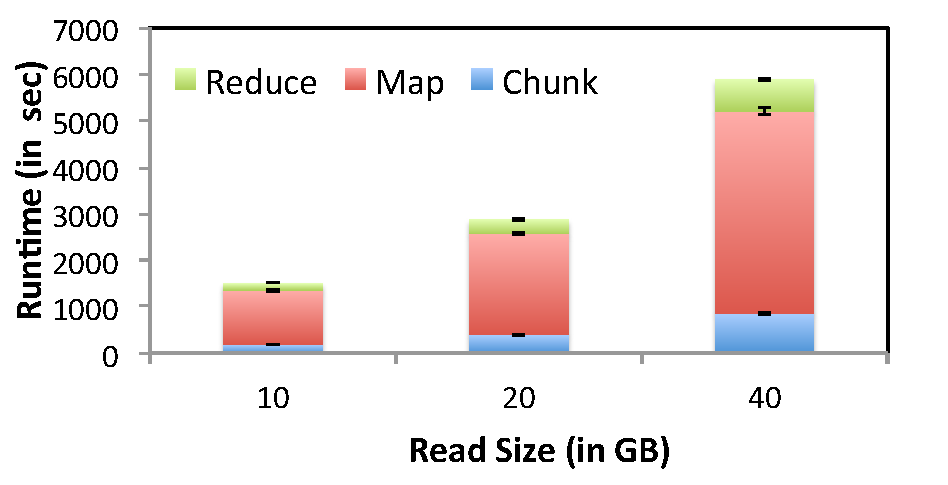
\includegraphics[scale=0.50]{figures/pj-smr-tts.pdf} 
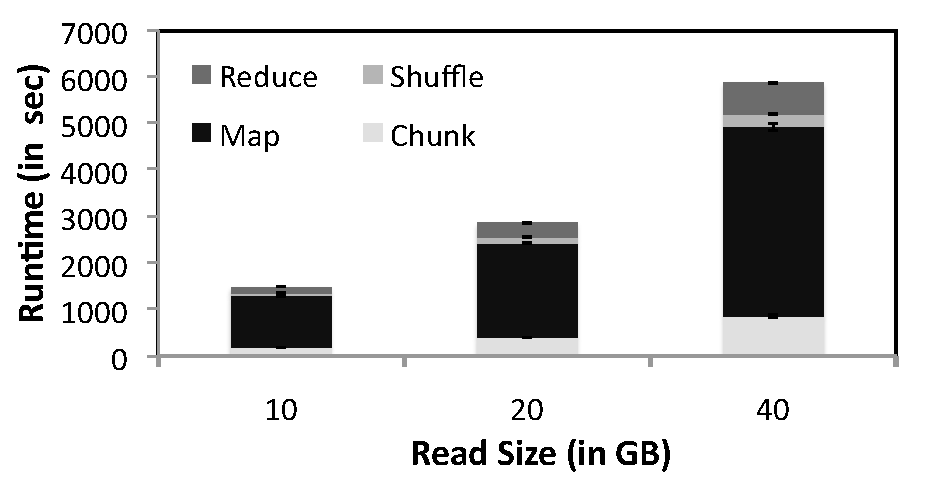
\includegraphics[scale=0.54]{figures/scale-out-bw2.pdf} 
\caption{\small Need of a scalable solution with increment of data
  volume.  Read size dependent time-to-solution is measured for
  MapReduce tasks of read alignment and duplicate read removal.  The
  number of nodes for this experiment,$N_{node}$ is 16(128 cores), the number of
  Workers, $N_W$ is 32, and the chunk size is set to contain 625000
  reads.  The number of Reducers is set to 8. BWA is used for read
  alignment.}
  \label{fig:read-size} 
\rev{Scale up.  The authors look at 32 mapper processes on what appear to be three configurations: 4 nodes with 4 workers (2 cores per worker), 4 nodes with 8 workers (1 core per worker), 8 nodes with 8 workers. It was unclear from the legend of Figure 2 how the extra 32 workers help in the third configuration.  Also, the last column in Table 2 does not match the legend as all nodes have 8 cores (and therefore 8 cores are only available with one worker per node?).  Figures 2 and 3 do not have entries in Table 2 (specifically the 16 node job).}

\rev{There is also little data on "scale out" (32 cores only on up to 4 nodes?)  For example, in this workshop a year ago there was a paper looking at a purely distributed file system framework based on "makeflow" and "work queue" that ran on up to 300 cores with 195X speedup with a similar map (megablast instead of a BW-based aligner) but a more complicated workflow.  Looking at the makeflow website this has been applied to BWA also and Weaver seems to be proposed as an abstraction similar to PMR (which as I understand is just a map and reduce running on SAGA?.  Their scaling seems heavily based on a hybrid distributed/multicore platform that I guess is a plus, but this puts restrictions on the type of systems usable for good performance.}

\end{figure}


%The good scalability with PMR shown in Fig~\ref{fig:scale-p-saga-mr}, as a matter of fact, appears to be helped by the characteristic nature of the target computational tasks.  The map phase, the read alignment is a single dominant step for the overall time-to-solution, and the %read alignment task is the most prominent example among a variety of NGS data analysis tasks that is suitable for data parallelization as well as task parallelization.  Note that the reduce phase task, duplicate read removal is also easy for parallelization primarily due to the fact %that to remove the duplicates needs only the local information, i.e. a single key or a small number of keys from the map phase results.  Despite of the simple nature, read alignment and duplicate read removal does provide an understanding of challenges for MapReduce-based %approaches for NGS data analytics.  For example, unlike the well-know word count problem, the map phase produces high volume of data size, indicating the low-aggregation problem, compared to the high-aggregation problem of the word counting\cite{weissman-mr-11}.  I%ndeed, the data management along with this feature should be considered carefully as indicated in Fig.~\ref{fig:read-size} with the 40 GB case that shows a significant portion of the processing time for chunking data.  Note that 40 GB is the entire data set from the RNA-Seq %experiment of interest.  Nonetheless, we note that the data management between the map phase and the reduce phase is reasonably handled by the Pilot framework for a single cluster or even a case for utilizing a couple of clusters as presented later.


\begin{figure}
 \centering
%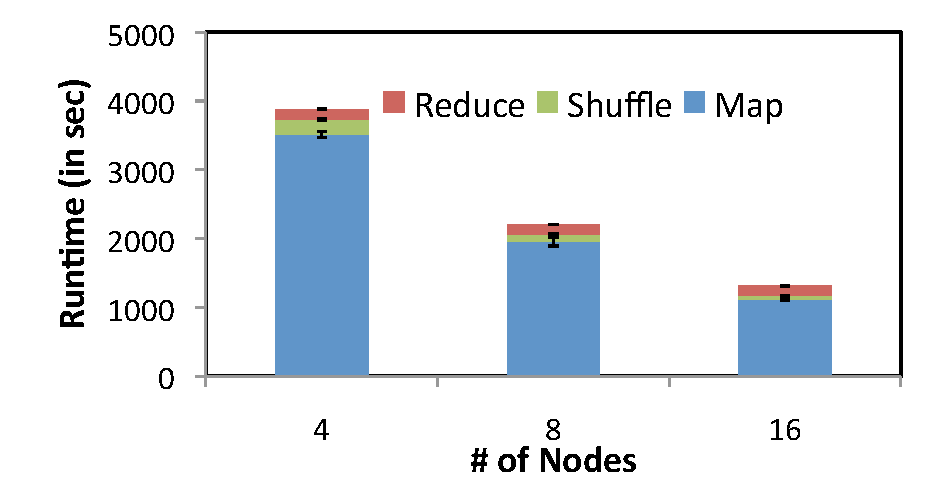
\includegraphics[scale=0.50]{figures/pj-smr-scale.pdf}
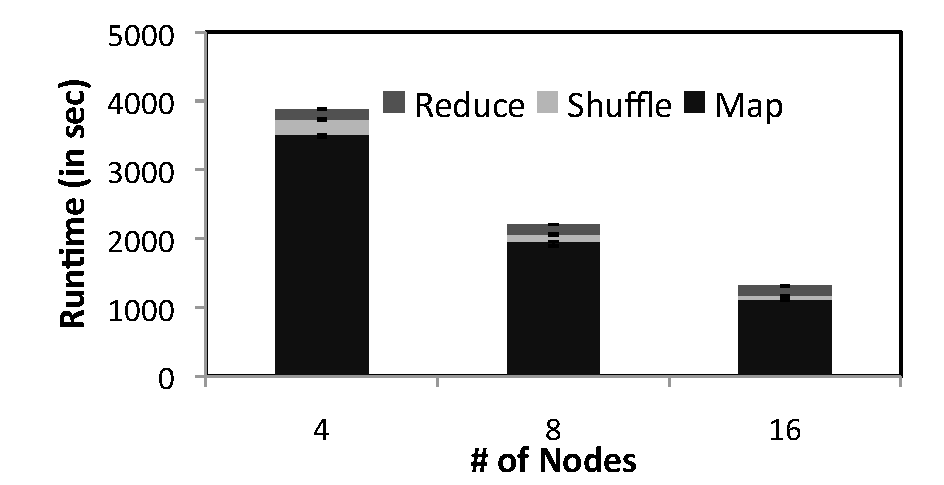
\includegraphics[scale=0.54]{figures/scale-up-bw.pdf} 
\caption{\small PMR scalability of a MapReduce-based computation for
  read alignment and duplicate read removal.  The number of Workers
  per node, $N_{W}/node$ is set to 2.  The input read file is 10GB,
  the number of Reducers is set to 8, The number of reads in a chunk
  is 625000. BWA is used for read alignment}
\alnote{I thought we don't include PMR only data}
\rev{ The authors look at 32 mapper processes on what appear to be three configurations: 4 nodes with 4 workers (2 cores per worker), 4 nodes with 8 workers (1 core per worker), 8 nodes with 8 workers.}

  \label{fig:scale-p-saga-mr} 
\end{figure}

\subsection{Extensibility}

\rev{ "what remains is experimental results with three mostly serial bioinformatics and their mapreduce implementations?  - can we include some mpi mapping applications
- novoalign/parallel bwa "}


We investigate the extensibility of PMR with two aligners -- BWA and
Bowtie.  One of the important reasons why multiple aligners are needed
is because of the difficulty of validation of an aligner used.  It is
well studied that each aligner implements different strategies to deal
with the requirement of computational loads, memory usage, and
sensitivity associated with decision on algorithms and computational
implementations of indexing, search, and match
tasks\cite{mapping-survey}.

Indeed, the decision of which aligner affects not only alignment
results but also investigate downstream analysis that aim to study
genome variation, transcriptome analysis, and DAN-protein
interactions. Therefore, it is not an overstatement to emphasize the
importance of supporting multiple tools as well as providing an
effective means for implementing such tools within a reasonably short
development period for infrastructure of NGS data.

Fig.~\ref{fig:tool_comp}, evaluates the performance of read alignment
in the map phase of both Hadoop and PMR based applications for Bowtie
and BWA aligners. Hadoop implementations - Crossbow uses Bowtie
aligner and Seqal uses BWA aligner.  Custom python wrappers to Bowtie
and BWA aligner are developed to execute alignment in the map phase of
PMR. In the evaluation, both Hadoop based implementations face the
problem of non-optimal configuration of Hadoop, i.e usage of shared
file system for HDFS, where as both local and distributed PMR perform
better than Hadoop map phase for both aligners. The PMR is extensible
and can support multiple NGS analytic tools.

Extending PMR to support new NGS analytic tools involve development of
simple map and reduce wrapper scripts to the tools. The wrapper
scripts could be developed in any language.  Hadoop streaming supports
this types of functionality but still involves complexity of managing
computational resources to maintain hadoop cluster.  PMR liberates the
user from the complex task of maintaining and acquiring computational
resources and executing map and reduce tasks on them.

\subsection{Parallelism} 
\alnote{Maybe parallelism would be a better caption.}
PMR supports multiple levels of parallelisms -- thread, task and
multiple-cores, and enables the flexible configurations of codes. For
example, BWA and Bowtie can be invoked to use varying number of
threads (fine-grained parallelism).  In Fig. \ref{fig:mulit-parallel},
we showed how such options could affect the performance.  Even
though it is feasible for other tools such as Seqal or Crossbow to
handle such options, the PMR approach of separating the runtime
environment (Pilot) from the code invocation in the Map and Reduce
phases, provides the capability of utilizing the fine-grained
parallelism along with the coarse grain parallelism provided by
MapReduce. The fine grain parallelism provided by Pilot-Job framework is demonstrated in replica exchange implementation \cite{repex_ptrsa}.

One of the advantages of PMR is it doesn't impose any restriction on
number of compute nodes that can be assigned to a particular map or
reduce task. This leads to a natural and native support for MPI-based
NGS tools. For example NovoalignMPI~\cite{novo-align} is a message
passing version of Novoalign, with claims of a more accurate aligner,
allows a single alignment process to use multiple compute nodes. The
MPI versions of Novoalign are more beneficial when large computing
infrastructures are available. Hadoop doesn't provide flexibility to
assign multiple compute nodes to a single compute task, thus leading
to an impedance mismatch between Hadoop MR and MPI based NGS analytic
tools.

%\subsection{Comparison to Hadoop-based Seqal and Crossbow}
% Compared to other areas, the computational biology community,
% specifically focusing on NGS data analysis, joined later for the use
% of MapReduce\cite{cloudburst}.  Nonetheless, there have been active
% works resulting in the programs listed in
% Table~\ref{table:mr-comparison}.

\subsubsection*{Related Work}

Cloudburst was one of the first generation tools in this field and
demonstrated the significant potential of the MapReduce model for NGS
data analysis.  After Cloudburst, Crossbow was developed by focusing
on better scalability using Hadoop streaming.  Compared to the two
Hadoop-based tools, GATK was introduced to address the general
parallel execution pattern across many NGS data analytics.  Recently,
the Seal package was announced in which Seqal is a utility for the
alignment and duplicate read removal.


\begin{figure}
 \centering
%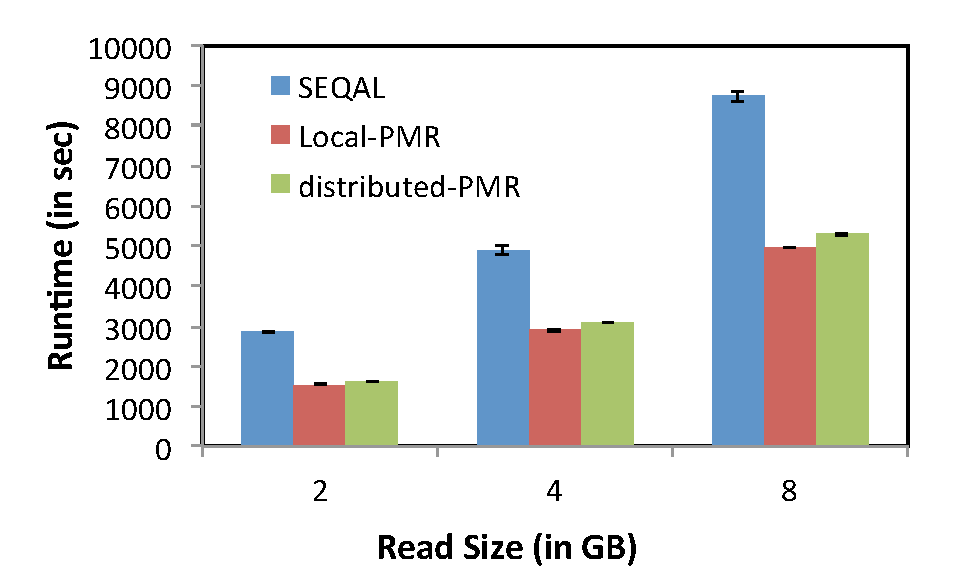
\includegraphics[scale=0.50]{figures/seqalvslocalpmr.pdf}
%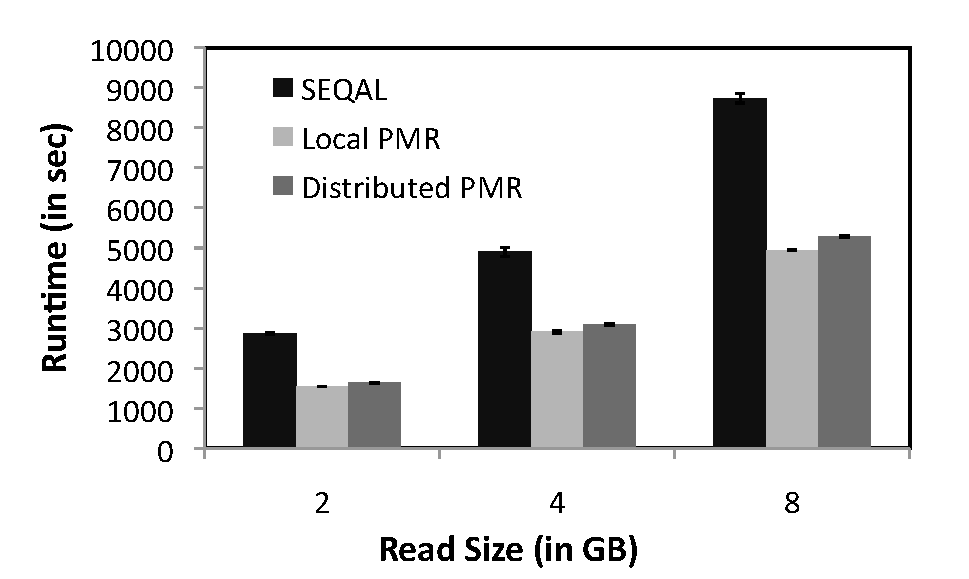
\includegraphics[scale=0.50]{figures/seqalvslocalpmr-bw.pdf}
%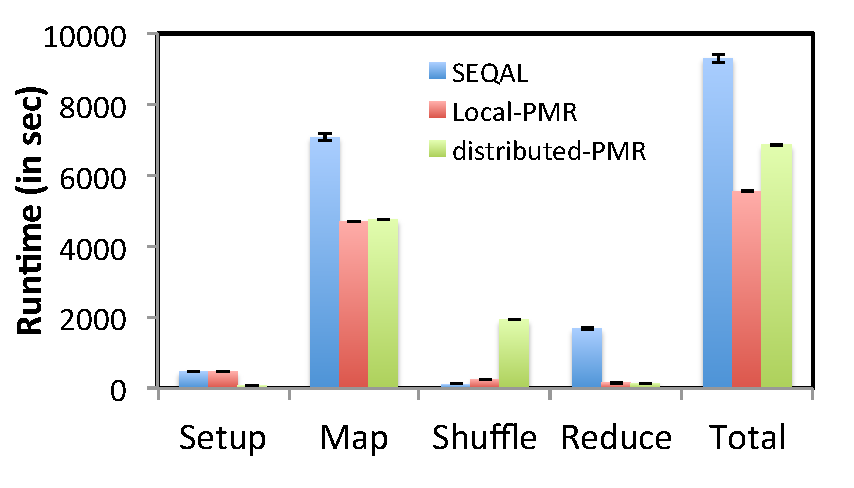
\includegraphics[scale=0.52]{figures/8GB_phasewisetimes.pdf}
%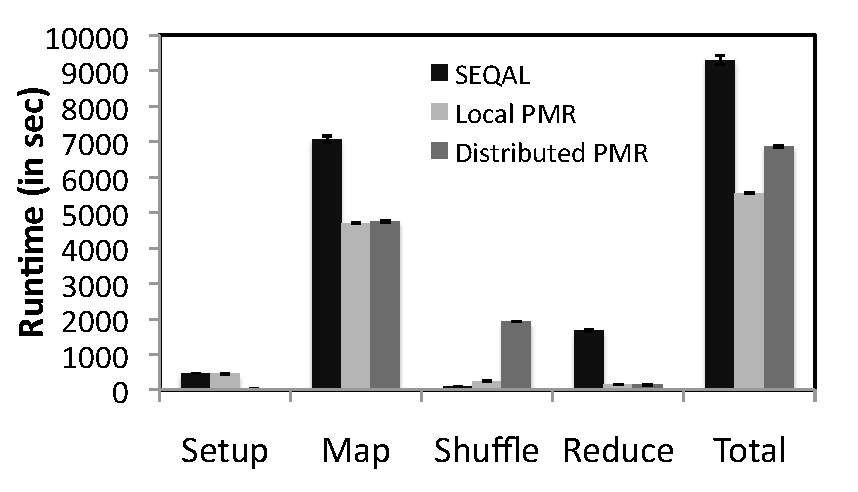
\includegraphics[scale=0.52]{figures/8GB_phasewisetimes-bw.pdf}
%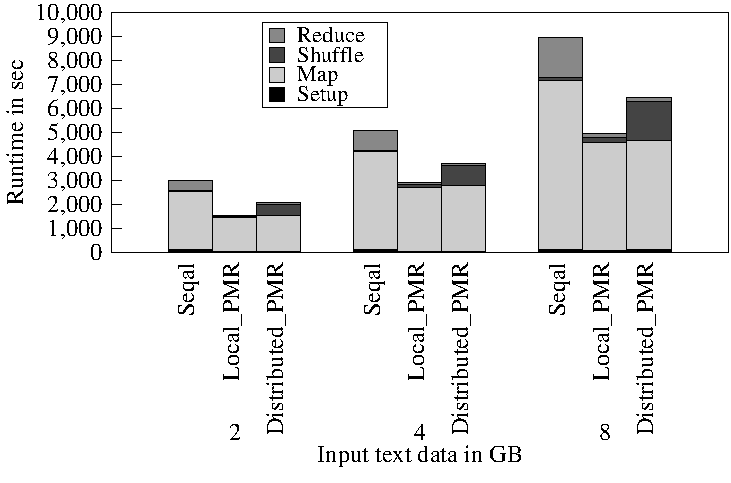
\includegraphics[scale=0.54]{figures/gs_seq_pmr_dpmr.pdf}
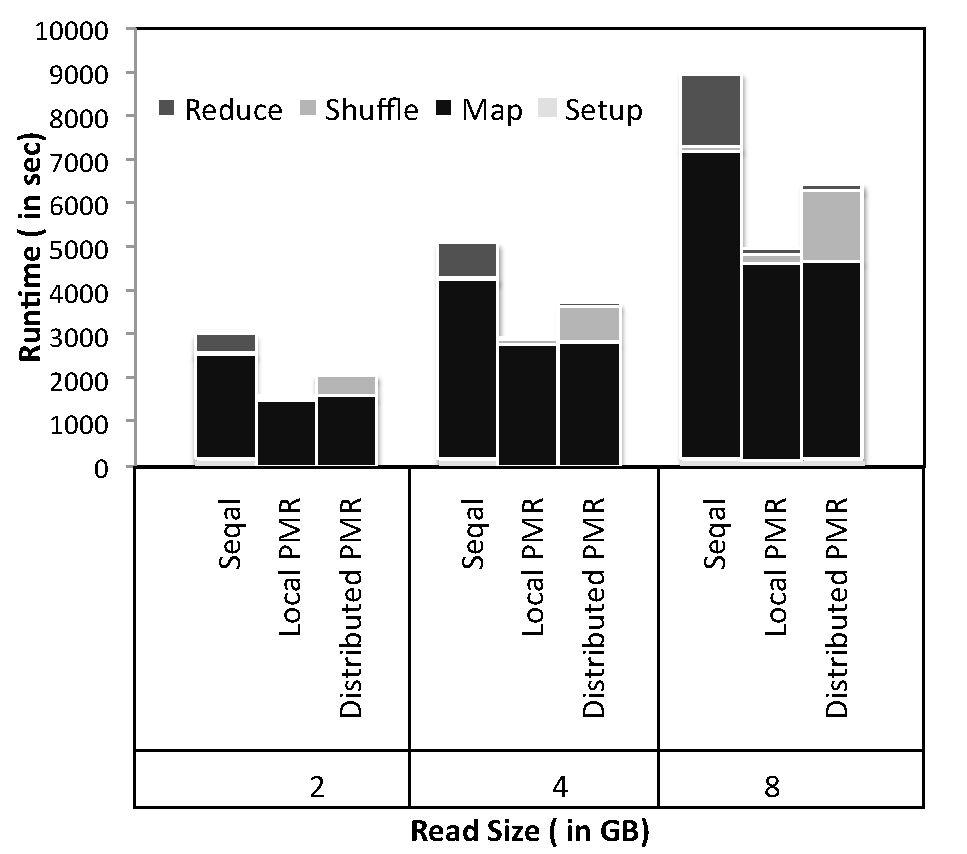
\includegraphics[scale=0.50]{figures/seqal_lprm_dpmr-full_3.pdf}


\caption{\small Comparison of the total time-to-solution for a MapReduce-based computation of alignment and duplicate read removal.  
Hadoop-based Seqal is compared to Local-PMR vs. distributed-PMR.  For this experiment, the number of Nodes, $N_{node}$ is 4, the number of Workers, $N_W$ is 8, the number of Reducers, $N_R$ is 8, and the number of reads in each chunk is 292,763. For the distributed-PMR, two machines of FutureGrid, Sierra and Hotel were used, whereas Sierra was used for other cases.}
\alnote{same analysis in in MR paper}

\rev{I don't think the Seqal comparisons are fair in that they use a shared filesystem (and scaling issues therein). It seems a little forced for comparison as there is the bottleneck of I/O for this tool.  On one hand you can view this as an advantage of their tool but I would expect similar "caching" for PMR (but maybe I am wrong) if they have the same number of chunks.}
\rev{The Seqal results in Fig4 are clearly biased in that the underlying file system was different.}
  \label{fig:comp_with_seqal_1} 
\secrev{However, the paper has 2 substantial flaws that limit its impact: (1) The performance measurements made against a vanilla Hadoop installation (Figures 4 \& 5) should be completely redone using proper Hadoop system.}
\end{figure}


\begin{figure} 
 \centering
%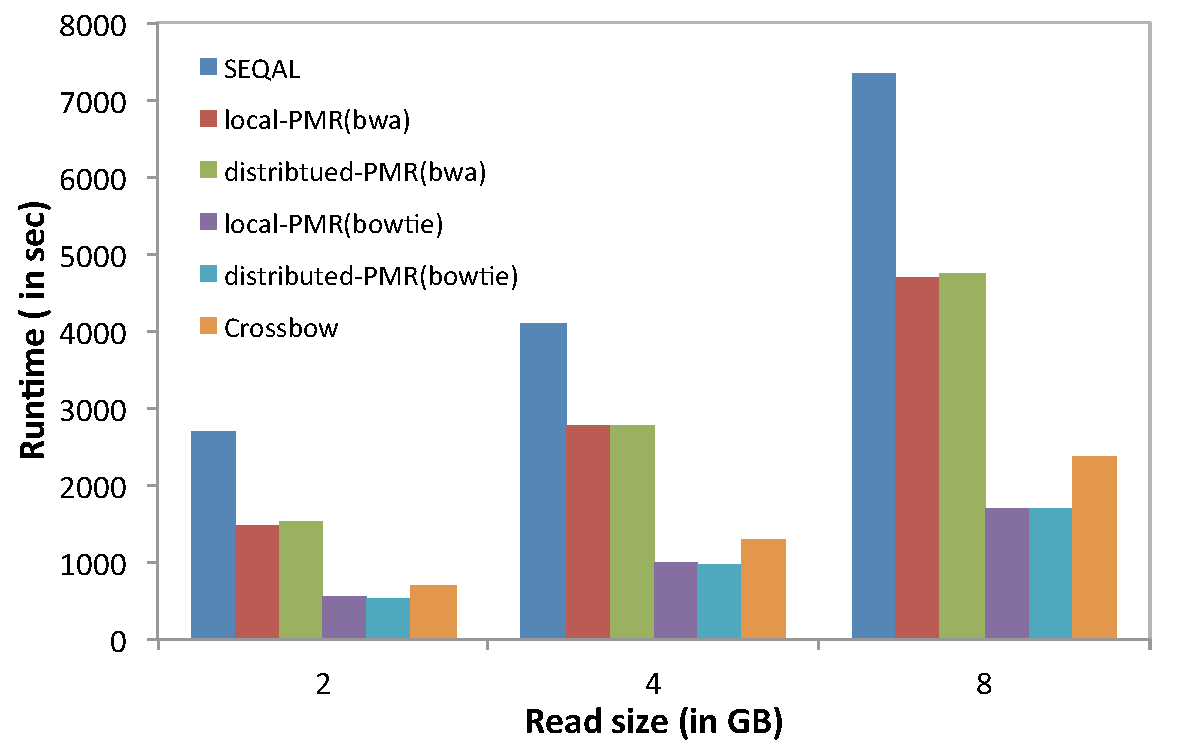
\includegraphics[scale=0.40]{figures/map_comp.pdf}
%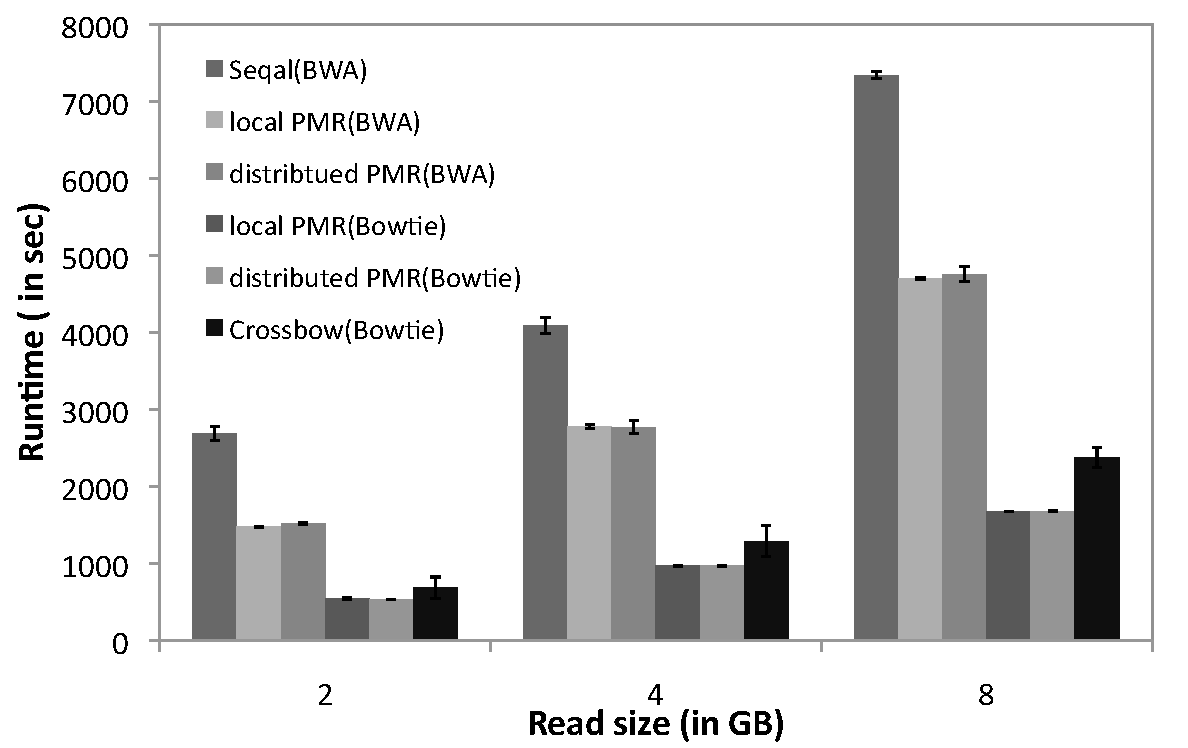
\includegraphics[scale=0.40]{figures/map_comp_bw.pdf}
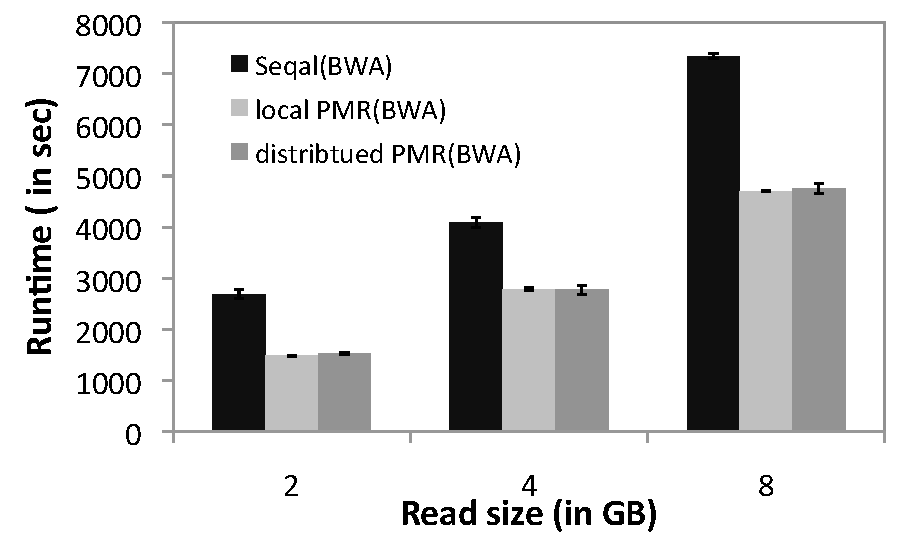
\includegraphics[scale=0.54]{figures/seqal_lpmr_dpmr.pdf}
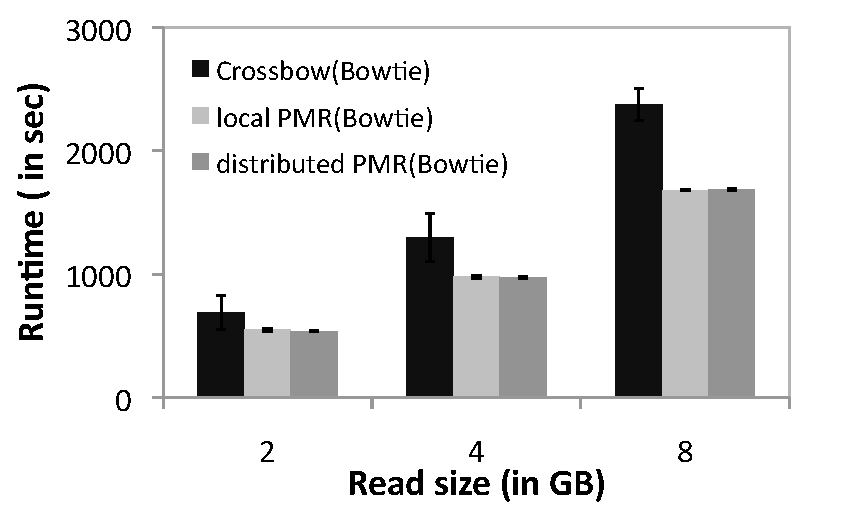
\includegraphics[scale=0.59]{figures/cb_lpmr_dpmr.pdf}
\caption{\small  Comparison of runtimes for the Map phase. The map phase of Seqal, Local-PMR(BWA), distributed-PMR(BWA), Local-PMR(Bowtie), distributed-PMR(Bowtie), and Crossbow(Bowtie) are compared.  The aligner used for each case is indicated in a parenthesis.  For this experiment, the number of nodes, $N_{node}$ is 4, the number of Workers, $N_W$ is 8, and the number of reads in each chunk is 292,763.  For the distributed-PMR, two machines of FutureGrid, Sierra and Hotel were used, whereas Sierra was used for other cases.}
  \label{fig:tool_comp} 

\rev{I can see where the authors are coming from with respect to the advantages of pilot jobs/ad hoc clouds but this is not described/tested in the paper; they only run on a few nodes they obtain from FutureGrid.  Further, I'm not convinced the map and reduce functional paradigm is better than, for example, something based on a straight-up master worker framework like some of the recent bioinformatics work with tools like Makeflow (to name only one).  The authors extend the framework to multiple tools but they still require a shared filesystem, which in practice severely limits "scale across" (see below and a bunch of recent papers)}
\rev{ Figure 5 was more problematic as it was unclear what crossbow they were comparing to.  Ideally, they should have used the latest one that does the same work as their pipeline.  In one part of the manuscript, they refer to it being also run using a shared FS and that the reduce step was not implemented.  With this in mind, what version was here and what does it mean that Crossbow is competitive with PMR for small collections of reads.  I would have much preferred discussion of the results (that differ from the previously submitted PMR framework) rather than an advertisement for PMR in the discussion.}
\secrev{(2) The authors should implement the reduce phase of Crossbow to truly measure the capability of distributed PMR. Without the reduce phase, the system is effectively a distributed batch scheduling system and does not demonstrate that distributed shuffle of large datasets is feasible. Until these two flaws are corrected, their major conclusions (PMR is a viable solution for scale-across NGS, and that PMR has advantages over Hadoop) are not proven.}
\pnote{The distributed PMR in pmr-2012 can be used here?}
\end{figure}


\begin{figure} 
 \centering
%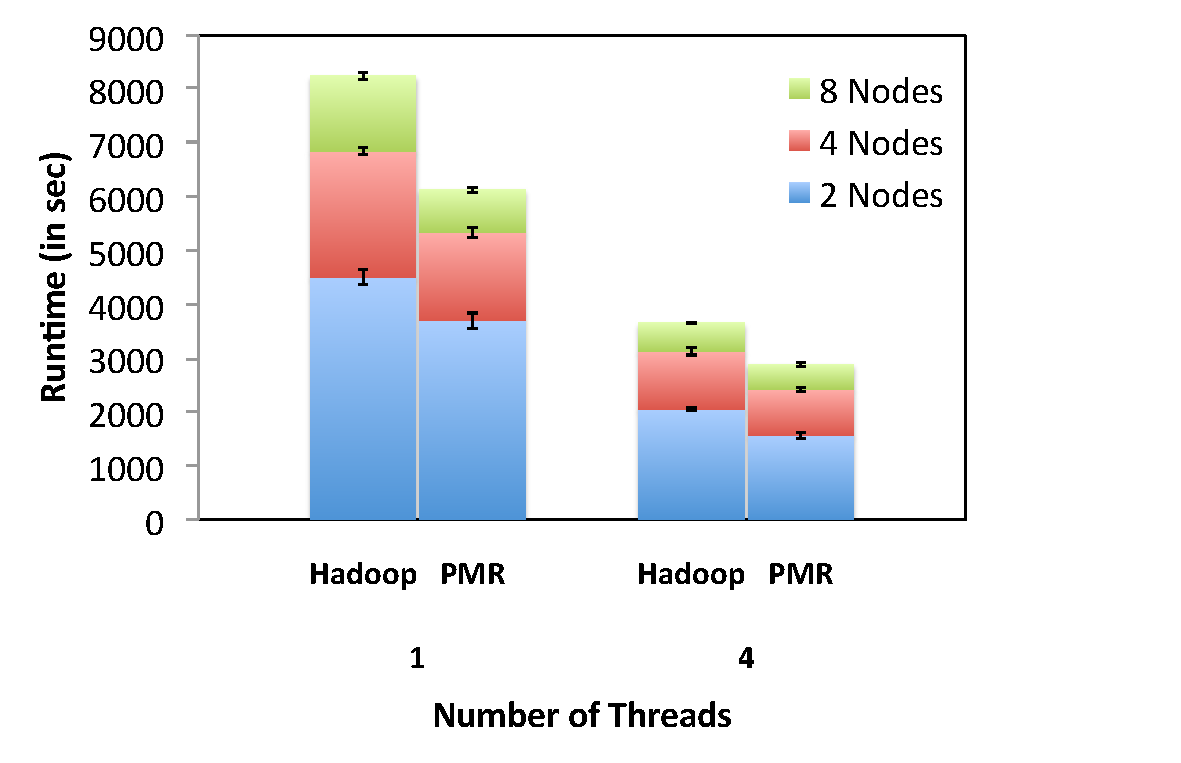
\includegraphics[scale=0.46]{figures/fig6_t.pdf}
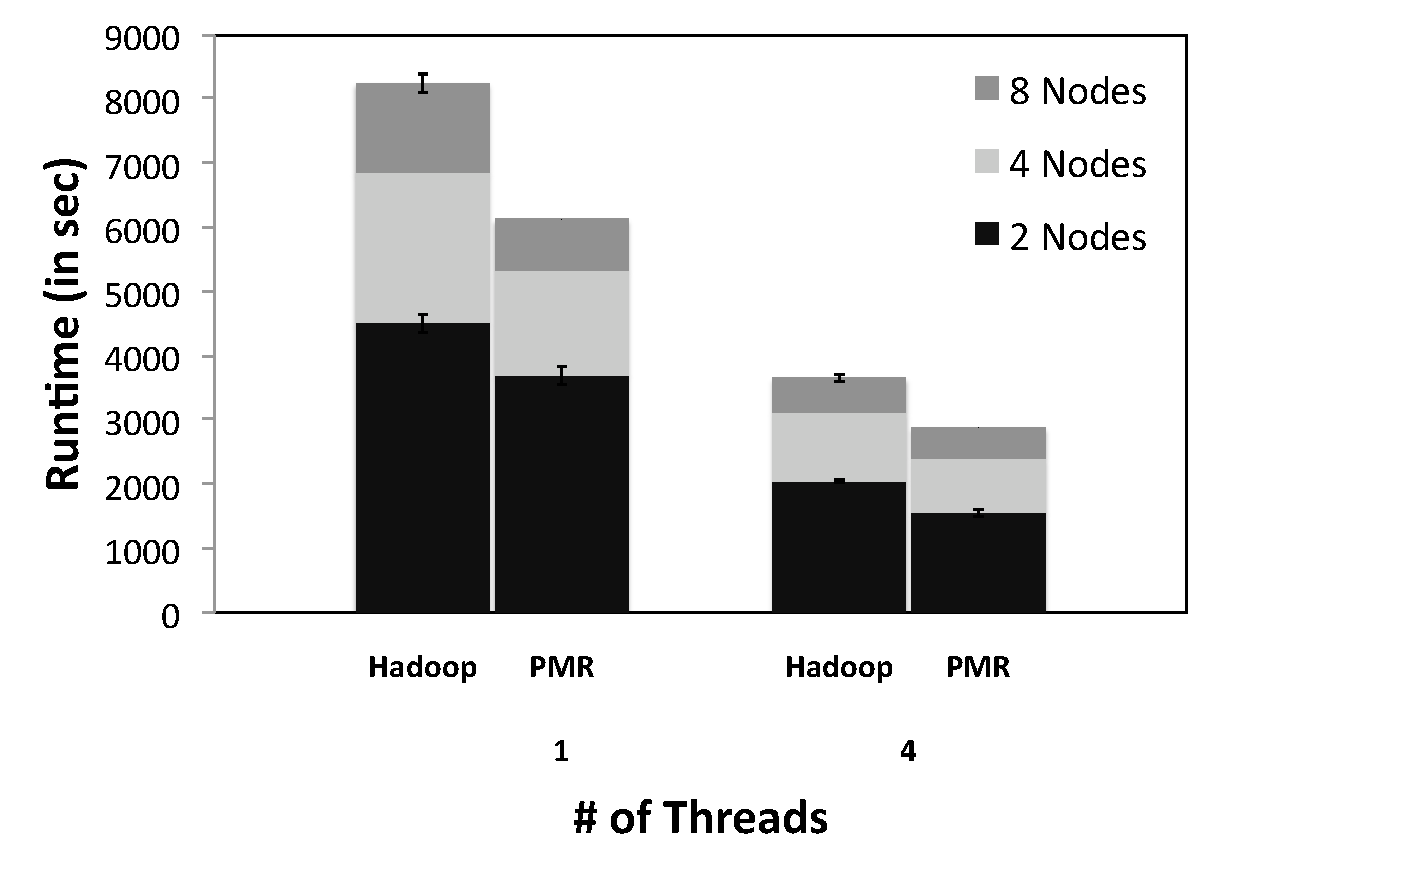
\includegraphics[scale=0.42]{figures/fig6_bw2.pdf}
\caption{\small The map phase runtimes of PMR(Bowtie) and Crossbow(Bowtie) are compared, by varying number of threads for each map task.  Number of workers/Node = 2 and input data size is 8 GB. The maximum number of cores assigned to a worker is 4, so we used 4 threads to achieve maximum fine-grain parallelism \alnote{What codes have been used here?}}
  \label{fig:mulit-parallel} 
\end{figure}

\section{Discussion}\label{sec:discussions}
\rev{In short, promising start -- especially when PMR is published -- but the authors should focus on scale up (more than 32 cores), showing scale across, and performing a better comparison with the state of the art such that current mapreduce tools are clearly run in a comparison (as opposed to edits) and that they use HDFS as intended.  Increasing the granularity such that the files can fit could help, maybe.}

% \textit{Computational Challenges for NGS data analysis, processing,
%   and downstream analysis}

DNA sequencing data generated by NGS
platforms\cite{metzker2010,1000genome,wang2009-natrevgen,alex2009,mcpherson2009}.
has resulted in a fundamental change in the amount of data that needs
to be analyzed. Such high-throughput technologies are able to provide
information about an entire genome or statistically meaningful number
of genomes of same species or related species.

% In the last several years, every area of biology and biomedical
% fields has witnessed a paradigm change with DNA sequencing data
% generated by NGS
% platforms\cite{metzker2010,1000genome,wang2009-natrevgen,alex2009,mcpherson2009}.
% Most importantly, these high-throughput technologies were able to
% provide the thorough information about an entire genome or
% statistically meaningful number of genomes of same species or
% related ones with enormously affordable cost, resulting in an influx
% of unprecedented amount of data.

While there have been algorithmic advances and a plethora of new
software tools by user-friendly interface via web-based tools, GUI
tools, or computing environments \cite{galaxy}, the end-to-end
development of scalable infrastructure is lagging.  MapReduce is a
widely employed programming model for parallelization of a large data
process; as reported by others with the tools listed in
Table~\ref{table:mr-comparison}, we observed that an efficient 
runtime environment for MapReduce such as that provided by PMR 
enables efficient methods for dealing with the required
scalability of NGS data analysis which comprises short reads alignment
and other following analysis such as duplicate read removal and SNP
finding.

%First, as shown in  Fig.~\ref{fig:read-size} and Fig.~\ref{fig:scale-p-saga-mr}. the map phase, read alignment, takes significantly more time than the task with the %reduce phase, duplicate read removal or other steps such as chunking input dta.  Secondly, the reduce phase task, like the map phase task, i.e. read alignment, additive.  %Here, the term additive means $f(X + Y) = f(X) + f(Y)$ where $X$ and $Y$ are input variables and $f$ represents the map or the reduce function.  On the contrary, SNP f%inding or other advanced NGS analysis are not in this type of analysis.   

% \textit{PMR, a viable solution for scale-across and extensible
%   framework for NGS data analytics}

\textit{PMR -- A viable solution for scale-across and extensible NGS
  analytics:} In fact, PMR not only supports scaling-across, it
provides some unique features, viz., support for distributed data
analysis and multiple tools that can each exploit multiple levels of
parallelism. %and extensible framework for NGS data analytics,
PMR provides an extensible runtime environment with which minimally
modified, yet standalone target tools are executed and the overall
workflow can be dynamically optimized by exploiting multiple levels of
parallelism. Furthermore, as indicated by results for BWA and Bowtie
for alignment, PMR allows further extensions of existing
implementation with other complementary tools or a flexible pipeline
development.  In fact, our primary goal behind this work is to develop
an integrative pipeline service for RNA-Seq data, and our development
presented in this work is indicative of preliminary progresses toward
such a goal.

\textit{PMR vs. Hadoop-based MapReduce tools: }The open source Hadoop
provides an ideal environment for the tools based on the MapReduce
programming model.  Perhaps, the ease of installation with commodity
hardware and the robust stability with fault-resiliency and easy
scalability could propel a wide acceptance of Hadoop.  Nonetheless,
Hadoop-based approaches find many hurdles in distributed contexts and
scenarios: for example, when scaling across multiple
clusters\cite{weissman-mr-11}, the execution of applications across
multi-nodes such as one using MPI, and the solutions involving the
limitations imposed by a current Hadoop implementation need to be
addressed.

% For example, due to limited scalability with Hadoop, discussions and
% suggestions for the next-generation Hadoop are being circulated in the
% community\cite{ng-hadoop-url}.\jhanote{What suggestions are these? Why
%   are they relevant here?}\jkimnote{this means that Hadoop is matured
%   but also aging...}  But 

As evidenced by the comparison of PMR-based read alignment and a
following analysis with two Hadoop-based tools -- Crossbow and SEAQL,
PMR-based implementations demonstrate scalability advantages over
Hadoop-based approaches. It is likely that future releases of Hadoop
address the distributed data scenarios too.

% It was reported that the overall performance of Hadoop-based
% MapReduce is determined by the unknown network performance and the
% connectivity between the data storage and the compute which are
% determined by characteristics of the cluster Hadoop is installed.
% The tight coupling between the MapReduce applications with
% underlying Hadoop causes unnecessary complexity when the
% optimization or the design of parallel execution is required.
% Secondly, it is not trivial to scale across different clusters.
% Many issues on the connectivity between two separate clusters
% including firewalls, different security policies, and potentially
% different administration structure are making difficult to extend
% Hadoop with other cluster systems.  Thirdly, it is a still ongoing
% concern that Hadoop's current implementation has obstacles from the
% scalability issue with the design with Namenode and Job tracker.
% The open source Hadoop is implemented with a job and task tracker:
% the job tracker is the central manager that dispatches map and
% reduce tasks to the nodes(nodes could be from multiple clusters) of
% the Hadoop cluster. On each node the task tracker is responsible for
% executing the respective tasks. The main limitation of this
% architecture is the fact that it intermixes both cluster resource
% management and application-level task managements. Thus, it is
% e.g. not easily possible to integrate Hadoop with another resource
% management tool, e.g. PBS or Torque. Also, the job tracker
% represents a single point of failure and scalability
% bottleneck. Another limitation is the latencies between machines
% should not be so big as HDFS uses Avro - an RPC-style protocol for
% communications.
%
%Collectively, PMR has edges in terms of flexibility and non-Hadoop-based architecture


\textit{DARE and beyond: }PMR-based NGS tools, implemented and
scrutinized in this work, were developed in conjunction with our
development of the runtime environment for dynamic applications,
Distributed Application Runtime Environment
(DARE)~\cite{dare-tg11,dare-ecmls11}.  DARE is a strategically
important component for the development of Science Gateway for NGS
data analytics and downstream analysis.  Under the design strategy of
DARE-based gateways, PMR-based tools were conceived to be a main
category of supporting execution patterns for parallel and distributed
task and data management.


\section*{Acknowledgement}

The project described was partially supported by Grant Numbers HPCOPS
NSF-OCI 0710874 award, NSF-ExTENCI (OCI-1007115) P20RR016456 from the
NIH National Center For Research Resources.  Important funding for
SAGA has been provided by the UK EPSRC grant number GR/D0766171/1 (via
OMII-UK) and the Cybertools project (PI Jha) NSF/LEQSF
(2007-10)-CyberRII-01.  Computing resources were made possible via NSF
TRAC award TG-MCB090174 and LONI resources.  This document was
developed with support from the National Science Foundation (NSF)
under Grant No.  0910812 to Indiana University for ``FutureGrid: An
Experimental, High-Performance Grid Test-bed.''  We also acknowledge
the Seal developer, Luca Pireddu for useful performance related
discussions, and Erik Flemington for allowing us to use his RNA-seq
data sets.

\bibliographystyle{unsrt}
\bibliography{compbio,saga}


\end{document}

Any opinions, ndings, and conclusions or recommendations expressed in
this material are those of the author(s) and do not necessarily
reflect the views.
